\section{Place Recognition Algorithm}
\label{sec:chap_slam_algo}

While there are a number of articles presenting place recognition algorithms using different sensors (e.g. camera~\citep{Cummins2011}, stereo-camera~\citep{Cadena2012}), the literature of such algorithms based solely on \gls*{3d} data is limited. For our place recognition analysis, we choose to evaluate on our datasets the state-of-the-art algorithm (at the time of the experiments) developed by~\citet{Steder2011b} on our datasets. We will first describe some fundamental concepts used for place recognition in Section~\ref{ssec:chap_slam_basics} and then we will give an overview of the Steder algorithm itself in Section~\ref{ssec:chap_slam_algo}. For the interested reader, the full details of the algorithm are available in~\citep{Steder2011b}.


\subsection{Fundamental Concepts}
\label{ssec:chap_slam_basics}

The following subsection is an introduction to basic concepts for understanding \gls*{3d} place recognition algorithms in general. In particular, conventional methods for representing and comparing \gls*{3d} acquisitions will be presented.

\subsubsection{Feature Keypoints and Descriptors}
\label{ssub:feature_keypoints_and_descriptors}

The first step in determining whether or not a place has been visited before, is to convert the sensor data into a format that is more convenient for identification. The generally-adopted representation is a vector of real numbers, called descriptor. This mathematical representation aims at being more compact than the original data while trying to capture significant characteristics from a recognition point of view.

A descriptor can be \emph{global}, meaning that it tries to capture information about the whole scan, or \emph{local}, meaning that it does the same but only for a specific subregion of the scan. When using local descriptors, one needs to select the keypoints around which the descriptors will be extracted. These keypoints can be at pre-determined and fixed locations (e.g. division in a simple grid) or selected using more refined algorithms. A common practice for the latter is to choose keypoints in so-called interesting regions which are often defined as regions of high gradient (e.g. edges, corners), as these region generally contains more information than smooth surfaces. Note that, for simplicity, we might use the term \textbf{features} as a more general term for keypoints and their respective descriptors in the remainder of this document.

The concepts of keypoints and descriptors first originated from the computer vision literature. More recently, they have been adapted for \gls*{3d} data. Some popular examples of features for both types of data are shown in Table~\ref{tab:features_examples}. Note that some algorithms propose solutions for both keypoints detection and descriptors (e.g. SIFT, NARF). However it is not mandatory to use them together as any combination is generally valid. While all features are different, they were all developed with the same goals in mind:
\begin{itemize}[label=$\bullet$,noitemsep,topsep=0pt]
    \item Distinctiveness: each feature should be easily differentiable with respect to others.
    \item Repeatability: the feature values should be stable under changes including:
        \begin{itemize}[label=$\circ$,noitemsep,topsep=0pt]
            \item Transformations: rigid transformation for point clouds and projective transformation for images, but also changes in the pose of the objects and/or the viewpoint.
            \item Noise: small variations in measurements (range/intensity) and occasional erroneous values (points/pixels).
            \item Resolution: the number of points or pixels representing a given area.
        \end{itemize}
\end{itemize}


\subsubsection{Range Image and NARF Feature}
\label{ssub:NARF Features and Range Image}

In this subsection, we present the NARF keypoints and descriptors, as well as the \gls*{3d} data representation on which they rely: the range image. We will see that the place recognition algorithm, presented in Section~\ref{ssec:chap_slam_algo}, relies on this \gls*{3d} representation to determine a matching score between scans.

Range images represent a \gls*{3d} data point by a pixel position (i.e x and y) and a range value. Note that the position of the pixel actually represents a horizontal and vertical angular position. For an omnidirectional \gls*{lidar} scan, the corresponding range image is a spherical projection of the points from the center of the sensor. Range images can be better defined by the constraints they must meet to be valid.

Firstly, converting a \gls*{3d} scan into a range image requires the acquisition to originate from a single view point and to have a single range value per pixel. It is therefore not possible to use point clouds acquired with multi-echoes \gls*{lidar}s or produced by merging multiple scans. Fortunately, the latter constraint is met in our datasets.

Secondly, every pixel in a range image must have a value. Since \gls*{lidar}s have a minimal and a maximal range, the data points outside this interval are ignored. Similarly, when a laser beam hits a highly absorbing or a reflecting surface at an angle, the sensor will not get any return. Such missing data points cause pixels of the range image to have no value, the latter are considered as far range (i.e. the maximum range of the sensor).

Finally, the resolution has to be adjusted so that each pixel of the resulting range image covers the same angular resolution vertically and horizontally. Images being discretized in pixels, the values of these can either be a weighted average of the laser beam ranges, or the value of the smaller range within his area, depending on the user preference. The converted scans have a dense and uniform representation similar to grayscale images, allowing the reuse of standard image processing techniques. Examples of range images can be seen in Figure~\ref{fig:chap_slam_range}.

\begin{figure}[H]
    \centering
    \subfloat[]{\label{fig:range_building}}{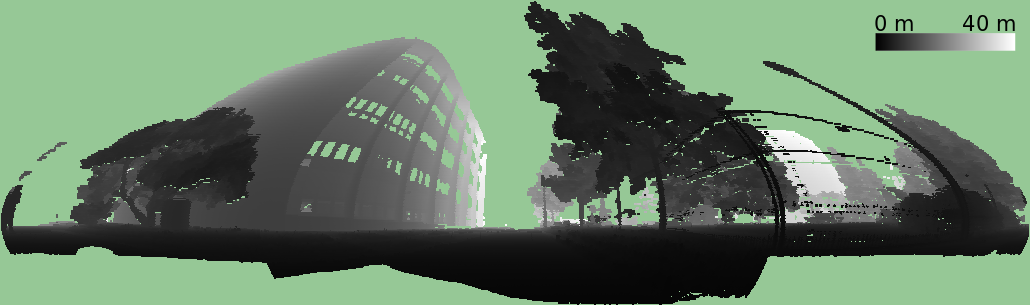
\includegraphics[width=0.995\linewidth]{img/chap_slam/range_building01_scale.png}}\\
    \subfloat[]{\label{fig:range_forest}}{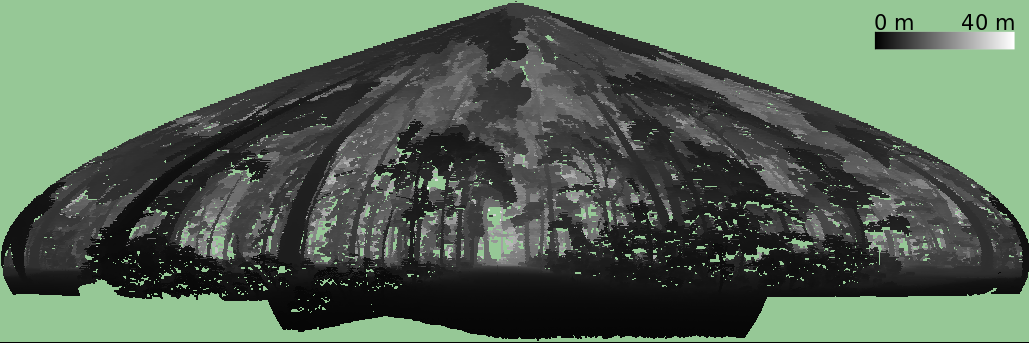
\includegraphics[width=0.995\linewidth]{img/chap_slam/range_forest01_scale.png}}
    \caption[Examples of range images from the two datasets.]{Examples of range images for the Structured-SICK dataset \protect\subref{fig:range_building} and the Unstructured-SICK dataset \protect\subref{fig:range_forest}. Note that objects appear distorted due to the projection on the plane. The background color (light green) corresponds to areas without laser return. All other pixels represent ranges between \SI{0}{\meter} (black) and \SI{40}{\meter} (white).}
    \label{fig:chap_slam_range}
\end{figure}

As indicated previously, feature keypoints are generally chosen in high gradient regions of the \gls*{3d} inputs. A problem arises when the input data is in the form of a point cloud, as it is impossible to distinguish edges caused by object boundaries from those caused by occlusion. Figure~\ref{fig:chap_slam_edges} present an example of a partial range image and the corresponding point cloud, where you can see edges caused by an object boundary and edges caused by the occlusion of this object. Edges caused by occlusions can generate meaningless keypoints and the descriptors built based on these keypoints leads to a poor representation of the environment, which can reduce the place recognition performance. This is particularly useful in our context of complex environments such as forest, because there are significant occlusions. The article describing the NARF features~\citep{Steder2011a} details how using range images allow to differentiate these two types of edges.

\begin{figure}[H]
    \centering
    %\subfloat[]{\label{fig:range_edge}}{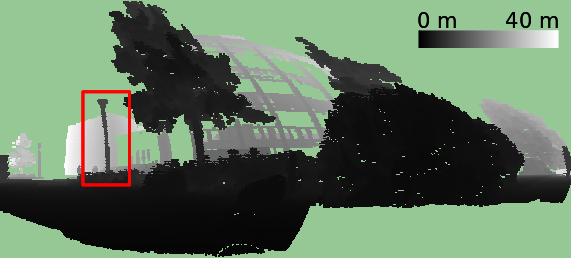
\includegraphics[width=0.507\linewidth]{img/chap_slam/range_building21_adjusted.png}}
    %\subfloat[]{\label{fig:pointcloud_edge}}{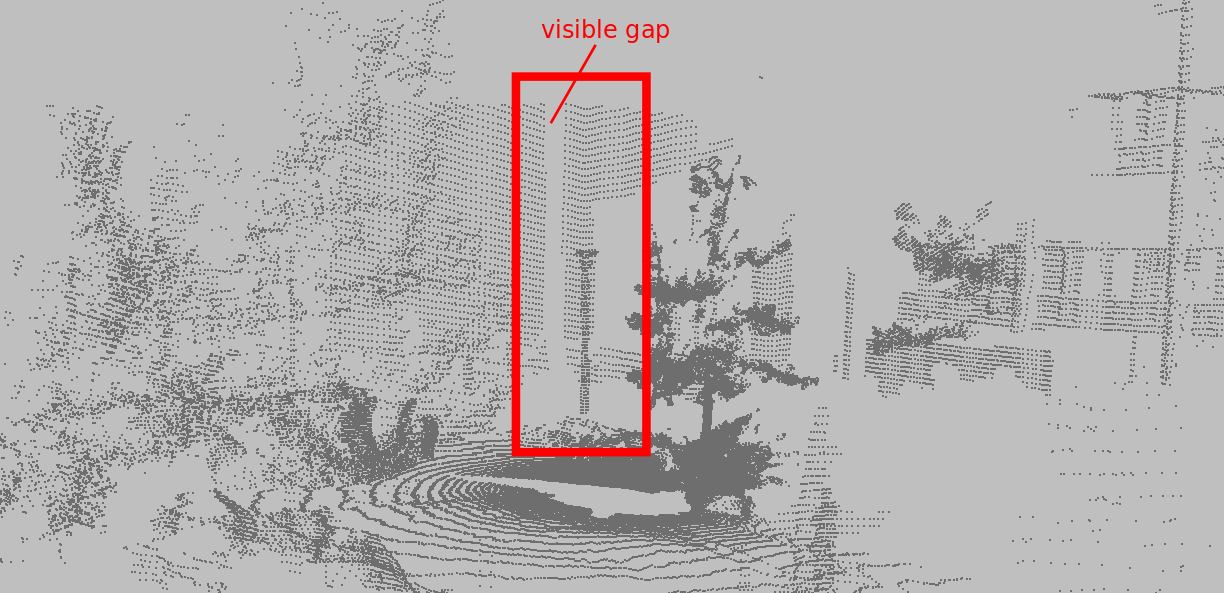
\includegraphics[width=0.473\linewidth]{img/chap_slam/pointcloud_building21.png}}
    \subfloat[]{\label{fig:range_edge}}{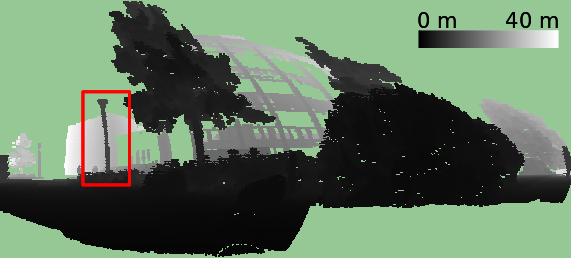
\includegraphics[width=\linewidth]{img/chap_slam/range_building21_adjusted.png}}\\
    \subfloat[]{\label{fig:pointcloud_edge}}{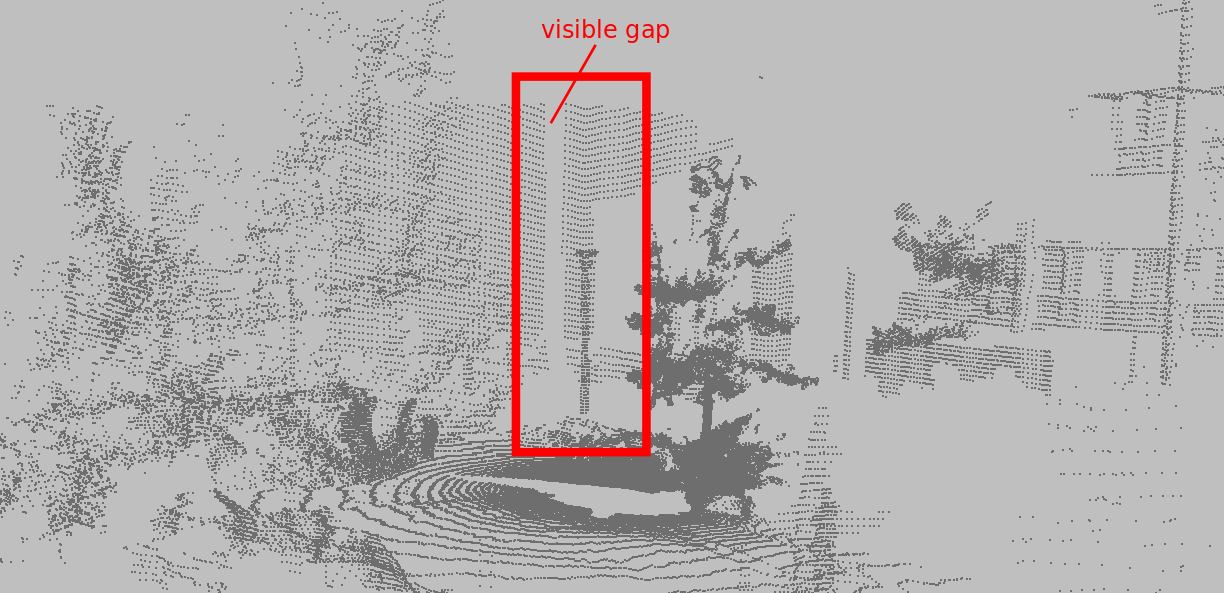
\includegraphics[width=\linewidth]{img/chap_slam/pointcloud_building21.png}}
    \caption[Example of a partial range image and the corresponding point cloud with an example of edge caused by an object border.]{Example of a partial range image \protect\subref{fig:range_edge} and the corresponding point cloud \protect\subref{fig:pointcloud_edge}. The red rectangle highlight a region of the environment where, from the robot point of view, a lamp post partially occludes a building wall. In the point cloud, this configuration leads to edges on both the lamp post boundary and the wall itself. In reality, the information contained in this scan does not allow to know what is behind the post and the edges of the wall are most likely artifacts caused by occlusion. In contrary, the range image is built taking into account the position of the sensor, thus allowing to consider only the boundary of the lamp post as edges and ignoring edges on the wall. Indeed, one can ignore the gap in the wall for the range image, as it is readily explained by the occlusion of the range image. Determining this occlusion is not possible by nature in a point cloud.}
    \label{fig:chap_slam_edges}
\end{figure}

\todo{Here I am in correction... the figure}
\todo{For sake of simplicity, we wont details how the (scalar) value for each green beam is computed, see article}
\todo{The histogram bin (descriptor value) with the maximum is the dominant orientation (unique orientation)}
\todo{The actual descriptor is visualized on the bottom. Each of the 20 cells of the descriptor corresponds to one of the beams (green) visualized in the patch, with two of the correspondences marked with arrows}

The last item to be discussed concerning the NARF features is the descriptor structure. In order to create this NARF descriptor, one must first compute the normal to the surface at the keypoint location. A star pattern, as shown in Figure~\ref{fig:narf_descriptor}, is then overlay on top of a small range image patch, as seen by an observer looking at the keypoint along the normal. Each beam of the star pattern corresponds to a single value in the final descriptor. This value captures how much the pixels changes under the beam (i.e. its gradient). A unique orientation around the normal is finally determined, to ensure that the NARF descriptor is rotation invariant\todo{How, largest value?}. An interesting characteristic of the NARF descriptors is that each of them encodes its own local coordinate system, allowing for a complete six degrees of freedom pose identification. This is possible due to the fact that we know the normal to the local surface patch and the unique orientation around the latter. Figure~\ref{fig:narf_descriptor} illustrates how descriptors are computed.

\begin{figure}[H]
    \centering
    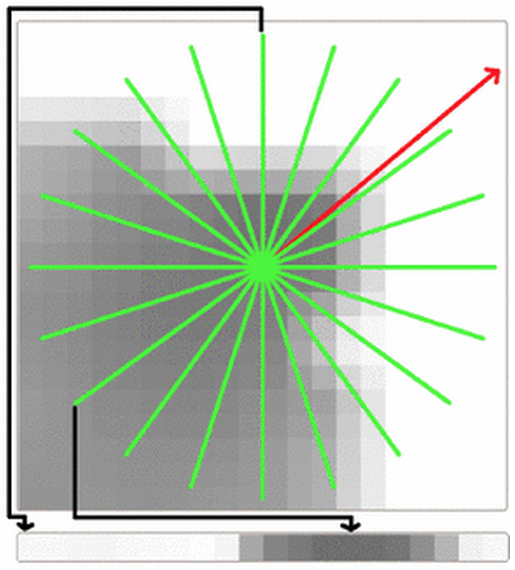
\includegraphics[width=0.4\linewidth]{img/chap_slam/narf.png}
    \caption[Illustration of a NARF descriptor calculated on a range image patch.]{Illustration of a NARF descriptor calculated on a range image patch. Each of the 20 green beams are represented by a single value in the descriptor vector. There are also 2 beams marked with arrows that show how pixels changes under them. In addition, the red arrow (pointing to the top right) show the extracted orientation around the normal of the patch. From~\cite{Steder2011a}.}
    \label{fig:narf_descriptor}
\end{figure}


\subsubsection{Scans Comparison}
\label{ssub:scans_comparison}

The last item to be discussed in this subsection is the method used to compare two scans. This is usually accomplished using the descriptors representing the scans. Since a descriptor is a vector of values representing the underlying data, two descriptors with very similar corresponding values should also represent similar entities (e.g. objects). Consequently, similarity between descriptors are generally computed using a simple distance metric (e.g. Euclidean distance, cosine distance).

The comparison between two scans using global descriptors is usually computationally inexpensive. Indeed, a single descriptor is computed for each scan and the comparison between two of them simply requires the computation of only one distance metric. Also note that for global descriptors, there is no such thing as keypoints and the geometric information is intrinsically included in the descriptor itself. A major drawback of such comparison approach is the high sensitivity to local changes of the environment, which may for example be caused by dynamic objects. This approach is also sensitive to small changes in position of the sensor of the sensor.

From a computational point of view, scans comparison based on local descriptors are more demanding. Indeed, besides having to calculate several keypoints and their associated descriptors, a method must be chosen to compare two scans over all features. In addition, the geometric relationships between features provides important cues about scans and may thus be considered to improve reliability of place recognition, albeit at a greater processing cost. Fortunately, using local features generally yield more robust results regarding local changes and also provides more comparison flexibility for the user. We will see a number of techniques for comparing scan using local features in the following paragraphs.

A first approach to compare \gls*{3d} scans with local descriptors consists in finding local descriptors correspondences between the scans. These correspondences are use to check if there is a valid transformation that aligns the scans. As we deal with data from real, noisy sensors, the vectors of real numbers representing the features (i.e. the descriptors) will never be exactly the same from one scan to another. A simple solution to this problem is to use the concept of nearest neighbor to identify the correspondences. One has to bear in mind that several descriptors may have no valid match due to background clutter or change in the view point. \cite[Section 7.1]{Lowe2004} describes how to remove most of those false matches by comparing the distance of the closest neighbor to that of the second-closest neighbor. The intuition is that this second best match is an incorrect one and using this ratio, only matches that have the closest neighbor significantly closer than the closest next match will be used, therefore improving reliability.

Once the corresponding descriptors between two scans have been identified, they are used to determine if there is a valid rigid \gls*{3d} transformation that align the underlying keypoints. The existence of such valid transformation serves as a first check on the similarity between two scans. This step also requires a criteria on the number (or ratio) of features correctly aligned, thereby identifying the scans as originating from the same place or not. This is generally achieved using the RANSAC algorithm~\citep{Fischler1981}. This rigid transformation estimation is computationally expensive, but has the advantage of being very discriminative. Additionally, it provides relative pose between scans, which is not possible using global descriptors. The relative pose can, for example, be used to determine odometry or during map creation process. Figure~\ref{fig:chap_slam_features_correspondences} shows keypoints from two scans of our dataset, as well as examples of correspondences.

A second solution, that speed up comparison when searching for potential matches between scans, is to represent the set of features of each scan by a \gls*{bow}~\citep{salton1983mcgill}. The concept of \gls*{bow} was first used for documents classification. In this context, \gls*{bow} represented a document by a vector of occurrence counts of a vocabulary without taking into account their ordering. In our case, the descriptors are made up of real numbers which allows for an infinity of them; therefore they cannot be used directly as words. The solution to this problem is to use a clustering algorithm such as k-means~\citep{MacQueen1967} to create groups that will represent words, a process known as \emph{quantization}. For instance, \citet{Cummins2008} present examples of visual words that typically correspond to the cross-piece of windows and other words that correspond to top-left corner of windows. An advantage of using k-means is that it is an unsupervised algorithm, meaning that no manual labeling effort is required. Because the \gls*{bow} approach avoids having to compare all potential feature correspondences between the scans, it significantly reduces the processing time. On the other hand, this method removes all information regarding the geometric configuration of keypoints in the scans, which might induce unwanted perceptual aliasing~\citep{Mariottini2011}. This is a rather general representation with for which the comparison is relatively fast to compute. Note that the visual dictionary is generally created in advance, in offline manner, using a large collection of local descriptors gathered under similar conditions and for similar scenes.

The chosen place recognition method will depends on several factors such as the available hardware resources, the desired processing time and the required reliability of the results. Using features correspondences along with geometric check is more computationally expensive than using the \gls*{bow} approach, but results are also more reliable. However, we will see in Section~\ref{ssec:chap_slam_algo} that it is possible to take advantage of the combined use of these methods.

\begin{figure}[H]
    \centering
    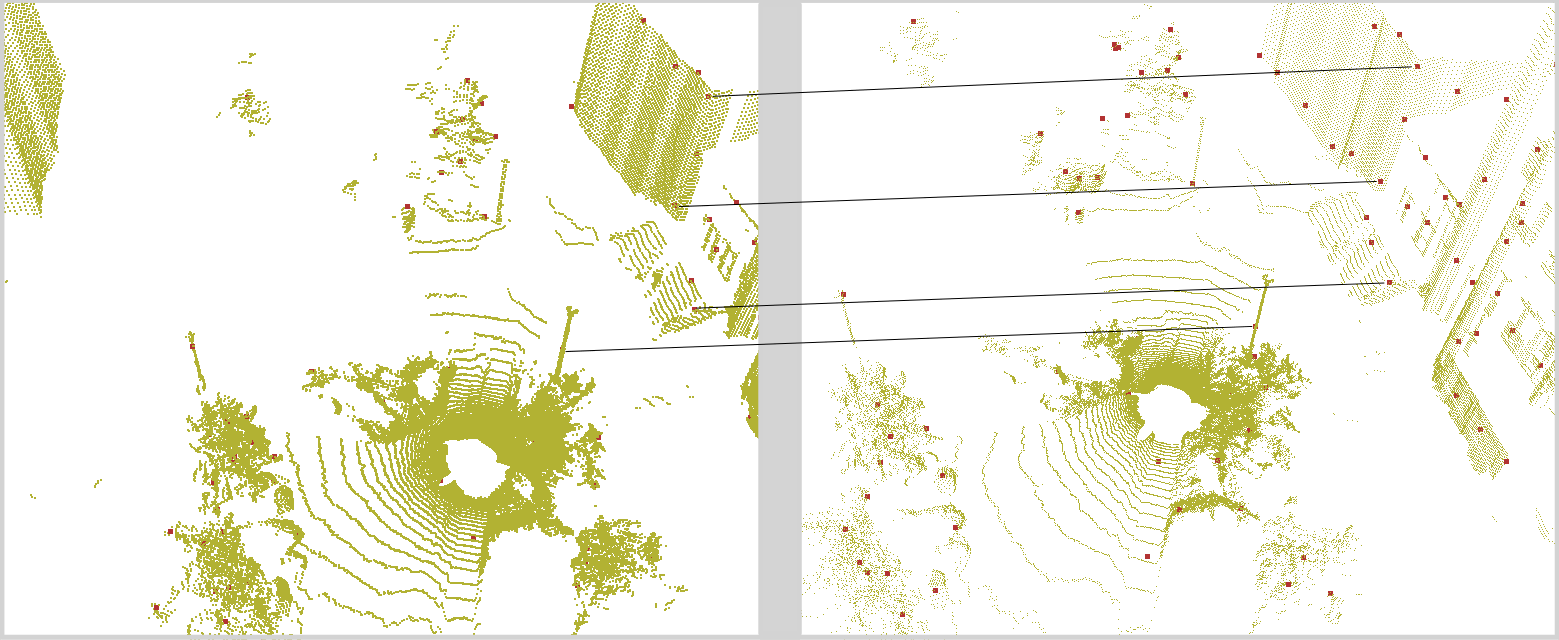
\includegraphics[width=0.995\linewidth]{img/chap_slam/features_line.png}\\
    \caption[Examples of NARF keypoints found for two different scans with examples of correspondences.]{Examples of NARF keypoints (red squares) found for two different scans of the structured dataset. Black lines illustrate examples of valid correspondences found across scans. These NARF keypoints show stability under changes, such as viewpoint, noise and resolution.}
    \label{fig:chap_slam_features_correspondences}
\end{figure}


\subsection{Overview of the Algorithm}
\label{ssec:chap_slam_algo}

\todo{This first paragraph act as a very broad explanation of the algorithm setup (general idea behind the protocol ?)... Rephrase the paragraph so this is clear}
The first requirement for the use of the place recognition algorithm is a set of 3D scans acquired at approximately regular interval by a robot equipped with an omnidirectional \gls*{lidar}. The initial set of scans for a given environment, dubbed scans database ($D$), acted as a representation of all known and visited places. Subsequent scans were used to determine if a match could be found in this database, and thus establish metrics such as precision and recall. This experimental procedure was repeated in different indoor and structured outdoor environments and with different \gls*{lidar}s.

In the original version of the algorithm \citep{Steder2010}, they compared a newly acquired scan ($z^*$) against all scans from the database ($z^1,...,z^{|D|}$), only using NARF features correspondences. As mentioned previously, these features encode a full \gls*{3d} pose, which in theory allow the determination of the transformation that align two scans based on a single features correspondence. This meant that there was as many candidate transformations as there was features correspondences between a newly acquired scan ($z^*$) and a single scan ($z^i$) from the database. Using a series of rules, a score was assigned to each of these transformations. This score reflected the system belief that this transformation was an actual match. The transformation having obtained the highest score is used to align $z^*$ with $z^i$.

Although this technique yielded high recognition rates, it required to compute a score for all candidate transformations (i.e. features correspondences) between the new scan and all the scans in the database. For real-time applications, this process is therefore too computationally expensive. An enhanced version of the algorithm, that we used for our experiments, was presented in~\cite{Steder2011b}. In this version, they first computed a \gls*{bow} representation for all scans. Based on this representation, they ordered all scans of the database from to the most similar (i.e. smallest Euclidean distance) to the least similar relative to the new scan. The calculation of scores for candidate transformations was then performed following this order. Consequently, the algorithm could be stopped when no more time was available and only matches that are less likely valid could be ignored. 

%Because the first version of the algorithm (i.e. \citep{Steder2010}) yield poor result in area with less distinctive structures, they added a self-similarity analysis. This is done using the score of the best non-identity transformation of a scan with respect to itself. By adjusting the score with respect to other scans, they can reduce the number of false positive. 

\begin{algorithm}
    \begin{algorithmic}[1]
        \INPUT
        \Statex $scanDatabase$ : the complete database of previous scans (range images)
        \Statex $newScan$ : the new scan to be matched and localized against the $scanDatabase$
        \OUTPUT
        \Statex $potentialMatches$ : set of (scanDatabase potential match for the newScan, best relative transformation, transformation score)
        \Statex

        \State $allBowDescriptors \gets \textsc{calculateAllDescriptorsForBagOfWords}(scanDatabase)$ \label{alg:bow_beginning}
        \State $dictionary \gets \textsc{createDictionaryForBagOfWords}(allBowDescriptors)$ \label{alg:dictionary}
        \State
        \Function{findPotentialMatches}{$scanDatabase$, $newScan$, $dictionary$}
        \State $newScanBow \gets \textsc{computeBagOfWords}(newScan, dictionary)$ \Comment{Keep scan reference} \label{alg:create_bow}
        \State \State $initSimilarities \gets \emptyset$ \Comment{Set of (scan reference, initial similarity score)}
        \ForAll{$scan \in scanDatabase$}
        \State $scanBow \gets \textsc{computeBagOfWords}(scan, dictionary)$ \label{alg:create_bow2}
        \State $initSimilarities.append(\textsc{getInitSimilarity}(scanBow, newScanBow))$ \label{alg:init_similarities}
        \EndFor
        \State $sortedSimilarities \gets \textsc{sortByScore}(initSimilarities)$ \label{alg:bow_end}

        \State
        \State $potentialMatches \gets \emptyset$, $i \gets 1$ \label{alg:correspondences_beginning}
        \State $newScanFeatures \gets \textsc{getScanFeatures}(newScan)$  \Comment{Each feature encodes the 3D pose} \label{alg:features_1}
        \While{$time \leq timeout$ \textbf{and} $i \leq |scanDatabase|$} \label{alg:timeout}
        \State $scan \gets \textsc{getScan}(sortedSimilarities_i)$
        \State $scanFeatures \gets \textsc{getScanFeatures}(scan)$ \Comment{Each feature encodes the 3D pose} \label{alg:features_2}
        \State $sortedMatches \gets \textsc{getSortedFeatureMatches}(scanFeatures, newScanFeatures)$ \label{alg:ordered_matches}

        \State
        \State $j \gets 1$, $bestTransfoScore = -\infty$, $bestTransfo \gets null$
        \While{$j \leq |sortedMatches|$ \textbf{and} $j \leq 2000$}
        \State $transfo,score \gets \textsc{computeMatchTransfoAndScore}(sortedMatches_j)$ \label{alg:transfo_score}
        \If{$score \geq scoreAcceptanceThreshold$ \textbf{and} $score \geq bestTransfoScore$}
        \State $bestTransfoScore \gets score$
        \State $bestTransfo \gets transfo$
        \EndIf
        \State $j \gets j + 1$
        \EndWhile

        \State
        \If{$bestTransfo \neq null$}
        \State $potentialMatches.append(scan, bestTransfo, bestTransfoScore)$
        \EndIf

        \State
        \State $i \gets i+1$
        \EndWhile \label{alg:correspondences_end}

        \State
        \State \Return{$potentialMatches$}
        \EndFunction
    \end{algorithmic}

    \caption{High Level Place Recognition Process~\citep{Steder2011b}}
    \label{alg:chap_slam_overview}
\end{algorithm}

Algorithm~\ref{alg:chap_slam_overview} presents a high level pseudocode of the general scan matching process. A first general note is that two sets of NARF features are extracted for each scan. This is because there is two general steps based on the features: the preordering of the scans from the database using the \gls*{bow} representation and the scoring of candidate transformations based on features correspondences. The section based on \gls*{bow} is presented from line~\ref{alg:bow_beginning} to~\ref{alg:bow_end} and uses a given set of feature parameters, while the second section for scoring candidate transformations is presented from line~\ref{alg:correspondences_beginning} to line~\ref{alg:correspondences_end} and use a different set of parameters. Table~\ref{tab:chap_slam_narf_parameters} shows the feature parameters used for those two cases. Authors explain that: \enquote{For the BoW approach a high number of features describing small parts of the environment is most useful\dots However, when matching a new query [scan] $z^*$ against [the database] $D$, a smaller number of more distinctive features is needed}.

\begin{table}[H]
    \centering
    \begin{tabular}{@{}lll@{}}
        \toprule
        \textbf{Parameters}  & \textbf{Values for \gls*{bow}} & \textbf{Values for the transformations scoring} \\
        \hline
        Max. feature counts & 2000                          & 200                                \\
        Descriptor size     & 36                            & 36                                 \\
        Support size        & 1/10 avg. range               & 1/5 avg. range                     \\
        \bottomrule
    \end{tabular}
    \caption[The set of NARF parameters used for the \gls*{bow} preordering step and the candidate transformations scoring step.]{The set of NARF parameters used for the \gls*{bow} preordering step and the candidate transformations scoring step. The support size is the radius around the keypoint, in the \gls*{3d} space, used to compute the descriptor. Note that the support size is represented by a proportion of the average range of all points in the database.}
    \label{tab:chap_slam_narf_parameters}
\end{table}

The first processing by the algorithm is the creation of the descriptors for all scans in the database (line~\ref{alg:bow_beginning}), which are then used to create the dictionary (line~\ref{alg:dictionary}). Note that, it would be possible to create a dictionary using a different set of scans (i.e. not the scans from the database) and/or update this dictionary according to some criteria, but this is not the case here. Once the descriptors have been produced, they are used to create 200 words (i.e clusters) using k-means. The output dictionary is then used to create a \gls*{bow} representation of each scan (line~\ref{alg:create_bow} and~\ref{alg:create_bow2}). Based on this representation, all scans from the database are stored in ascending order, according to the Euclidean distance between their vectors representing word counts and the vector of the input scan (line~\ref{alg:init_similarities}). The intuition is that scans with a small distance between them are more likely to originate from the same place. They will therefore be processed first during the next step, as they are the most promising. This greedy approach is required because of the timeout (line~\ref{alg:timeout}) that might prevent the last scans to be processed.

The features created using the set of parameters for candidate transformation scoring are used to find potential transformations between each database scan and the input scan ($newScan$). As indicated previously, each NARF feature encodes its full 3D pose, therefore a single features match allows the determination of the transformation that should align the two scans. Since there is 2000 features per scan, there are up to 2000 transformations to be tested for each scan from the database. To determine the corresponding features, all pairs of features (one from the processed database scan and one from the input scan) are ordered by ascending order according to their Manhattan (i.e. L1) distance in the space of descriptors. Again, descriptors with a small distance between them are more similar and therefore more likely to be valid matches; they are therefore prioritized for the scoring process.

Although the candidate transformation scoring process is not detailed (line~\ref{alg:transfo_score}), it is an important part of the place recognition framework that we will briefly describe here. As explained in Section~\ref{ssec:chap_slam_basics}, range images are linked to the \gls*{lidar} sensor model. Each pixel represents the range from the origin of the sensor to the target for a specific angular position. Considering that the step of aligning the input scan ($z^*$) with the database scan ($z^i$) is already completed, one can easily determine where the pixel $p^*$ from $z^*$ will fall into $z^i$, as well as the range value it should have. Let $r^*$ be the range of the processed point in $z^*$ and $r^i$ the range of the corresponding point in $z^i$. A score representing how good $r^*$ is explained by $r^i$ can be computed according to different scenarios presented in Table~\ref{tab:chap_slam_scoring_scenarios}.

This scoring process is applied to all validation points and the final score for the candidate transformation is a function (see~\citep[Equation~1]{Steder2011b}) of those individual point scores. To avoid a small error in the transformation to cause low score, they not only consider the exact matching points, but also neighbors in small pixel radius.

Finally, note that the set of validation point is a subsample of points, since using all points from the input scan would be too expensive to compute. Instead, the set of points used is fixed to a predefined size (200 points for the experiments). Points are chosen to evenly cover the 3D space and to have some significance in the scene. 

\begin{table}[H]
    \centering
    \begin{tabular}{@{}p{0.17\textwidth}p{0.54\textwidth}p{0.23\textwidth}@{}}
        \toprule % Observation = database, Prediction = input scan
        \textbf{Ranges relation}         & \textbf{Interpretation}                                                                                                    & \textbf{Effect on the score} \\
        \hline
        $|r^i - r^*| < \Delta r_{max}$   & The difference between $r^i$ and $r^*$ is within the confidence range. This is most likely a valid correspondence.      & Increase $\propto 1-\frac{|r^i-r^*|}{\Delta r_{max}}$ \\
        $r^i - r^* > \Delta r_{max}$     & The range of the pixel from the database scan is larger than the corresponding pixel from the input scan. This could be caused by a dynamic or partially transparent obstacle, but this is more likely caused by a wrong transformation. & Highly decrease \\
        $r^i - r^* < -\Delta r_{max}$    & The range of the pixel from the database scan is smaller than the range of the corresponding pixel from the input scan, leading to two subcases : & \\
                                         & 1) A known obstacle in the database scan hides the pixel from the input scan.                                           & Slightly decrease \\
                                         & 2) The pixel does not exist in the input scan. This could be caused by an unseen or dynamic obstacle, but it is more likely caused by a wrong transformation.       & Highly decrease \\
        $\nexists : r^i \correspond r^*$ & The pixel from the input scan ends up outside of the database scan limit (i.e. there is no reference for this point).   & Slightly decrease \\
        $r^i \ge MAX$                    & The range of the pixel from the database scan is larger or equal to the sensor maximum reading range, leading to two subcases : & \\
                                         & 1) Based on the value of the input scan pixel, the corresponding pixel of the database should be closer to the sensor.  & Highly decrease \\
                                         & 2) The pixel of the database scan moved away from the sensor and could possibly be out of range.                        & Modestly decrease \\
        \bottomrule
    \end{tabular}
    \caption[A summary of the different scenarios for scoring corresponding pixels of the range images.]{A summary of the different considered scenarios for scoring corresponding pixels of the range images. The range of the pixel from the input scan is $r^*$ and the range of the corresponding pixel from the database scan is $r^i$. Note that, $\Delta r_{max}$ is a positive value representing the maximum difference in range between the pixels to be considered as a valid correspondence and $MAX$ is the maximum range for the given sensor.}
    \label{tab:chap_slam_scoring_scenarios}
\end{table}

This concludes the general overview of the place recognition algorithm~\citep{Steder2011b}. In the following section, we will explain how we used it to compare the impact of different environments on the recognition performance.
